\documentclass[10pt,a4paper]{article}
\usepackage[utf8]{inputenc}
\usepackage{amsmath}
\usepackage{amsfonts}
\usepackage{amssymb}
\usepackage{german}
\usepackage{fancyhdr}
\usepackage{graphicx}
\usepackage{geometry}
\usepackage{listings}
\usepackage{hyperref}
\usepackage[onehalfspacing]{setspace}
\usepackage{color}
\usepackage[usenames,dvipsnames]{xcolor}
\usepackage{DejaVuSans}
\usepackage[T1]{fontenc}
\renewcommand*{\familydefault}{\sfdefault}
\geometry{verbose,a4paper,tmargin=35mm,bmargin=35mm,lmargin=25mm,rmargin=25mm}
\author{Dominik Heeb, Fabian Keller}
\title{Projektplan Semesterarbeit}
\pagestyle{fancy}
\fancyhead{}
\fancyhead[L]{DPC Alrogithmus Vector Clock}
\fancyhead[R]{Domink Heeb, Fabian Keller}
\fancyfoot{}
\fancyfoot[R]{Seite \thepage}

\definecolor{bluekeywords}{rgb}{0,0,1}
\definecolor{greencomments}{rgb}{0,0.5,0}
\definecolor{redstrings}{rgb}{0.64,0.08,0.08}
\definecolor{xmlcomments}{rgb}{0.5,0.5,0.5}
\definecolor{types}{rgb}{0.17,0.57,0.68}
\lstset{language=[Sharp]C,
captionpos=b,
%numbers=left, %Nummerierung
%numberstyle=\tiny, % kleine Zeilennummern
%frame=lines, % Oberhalb und unterhalb des Listings ist eine Linie
showspaces=false,
showtabs=false,
breaklines=true,
showstringspaces=false,
breakatwhitespace=true,
escapeinside={(*@}{@*)},
commentstyle=\color{greencomments},
morekeywords={partial, var, value, get, set},
keywordstyle=\color{bluekeywords},
stringstyle=\color{redstrings},
basicstyle=\ttfamily\normalsize,}

\begin{document}
\begin{titlepage}
	\begin{Huge}
		\begin{center}
				Algorithmus Vector Clock \\Dynamic Parallel Checker\\[2.0cm]
		\end{center}
	\end{Huge}
	
	\begin{center}
		\begin{Large}
				by Dominik Heeb, Fabian Keller\\[1.0cm]
		\end{Large}
		\begin{large}
				Betreuer: Prof. Dr. Luc Bläser
		\end{large}
	\end{center}
\end{titlepage}

\newpage
\tableofcontents 
\newpage

\section{Allgemein}
\subsection{Vector Clock}
\begin{flushleft}
Die Vektor Clock ist ein Vorgehen um einzelnen Messages oder Events einen eindeutigen Zeitstempel zuzuweisen. Somit eine logische Uhr, die es erlaubt in einem Verteilten System (bei uns mehreren Threads) die Ereignisse aufgrund des Zeitstempels einer Kausalordnung zuzuweisen und insbesondere die Nebenläufigkeit von Ereignissen zu ermitteln.
\\[0.5cm]Link:\href{https://de.wikipedia.org/wiki/Vektoruhr}{Wikipedia - Vektor clock}
\end{flushleft}
\subsection{Happened-Before Beziehung}
\begin{flushleft}
Ist eine Beziehung zwischen zwei Zeitpunkten. Mit Hilfe der Vektor Clock wird jedem Ereignis ein Zeitstempel zugewiesen und anschliessend herausgefunden in welcher Happened-Before Beziehung die beiden Zeitstempel stehen.\\
Eigenschaften der Happened-Before Beziehung:
\begin{itemize}
\item Auf demselben Prozess: a -> b wenn die Zeit von a < b. (Zeit ist durch lokale Uhr gegeben)
\item Wenn ein Prozess eine Nachricht zu einem anderen Prozess senden, dann a -> b wenn a der Sender und b der Empfänger ist.
\item Für drei Ereignisse a, b, c, wenn a -> b und b -> c, dann a -> c (Transitivität)
\end{itemize}
In unserem speziellen Fall arbeiten wir mit dem Vergleich der einzelnen Elementen des Vektors. Dabei gibt es zwei verschiedene Beziehungen die zwei Ereignisse miteinander haben können:\\
\textit{\textbf{Happened-Before}\\[0.2cm]}
\begin{tabular}{ c c }
  (x1, x2, x3) -> (y1, y2, y3) & (y1, y2, y3) -> (x1, x2, x3) \\
  y1 >= x1 & x1 >= y1 \\
  y2 >= x2 & x2 >= y2 \\
  y3 >= x3 & x3 >= y3 \\[0.2cm]
\end{tabular}
\\Jedes Elemente eines Vektors ist grösser oder gleich dem Elemente des selben Threads im zweiten Vektor. Dadurch hat eine Synchronisation stattgefunden und es kann eine Aussage zu der Happened-Before Beziehung gemacht werden.\\
\textit{\textbf{Concurrent}\\}
Wenn keine Aussage über die Happened-Before Beziehung gemacht werden kann, sprich der erste Zustand nicht gilt, sind die Ereignisse Concurrent. D.h. sie können gleichzeitig abgelaufen sein und daher für den Dynamic Parallel Checker interessant.\\
\end{flushleft}
\newpage
\section{Vektor Clock Algorithmus}
\subsection{Beispiel}

\begin{flushleft}
Der Vektor Clock Algorithmus wird in diesem Kapitel mit Hilfe von folgendem C\# Code genauer erläutert.\\
\begin{singlespace}
\begin{lstlisting}
object a = 1;				// main thread1 (T1)
object b = 1;
b = 2;
Task.Factory.StartNew(() =>		// start thread2 (T2)
{
	lock(b) {
		b = 3;
	}
	b = 4;
	lock(a) {
		Console.WriteLine(a);
	}
});
Task.Factory.StartNew(() =>		// start thread3 (T3)
{
	lock(a) {
		a = 2;
	}
	b = 5;
	lock(b) {
		Console.WriteLine(b);
	}
})
lock(a) {
	a = 3;
}
lock(b) {
	b = 6;
}
Console.WriteLine(a);
\end{lstlisting}
\end{singlespace}
\end{flushleft}

\begin{flushleft}
Diese Beispielfunktion aus Sicht der Dynamic Parallel Checker sieht wie folgt aus: (Nur Lese-, Schreib-, Lock- und Unlockzugriffe auf Ressourcen)\\[0.5cm]
	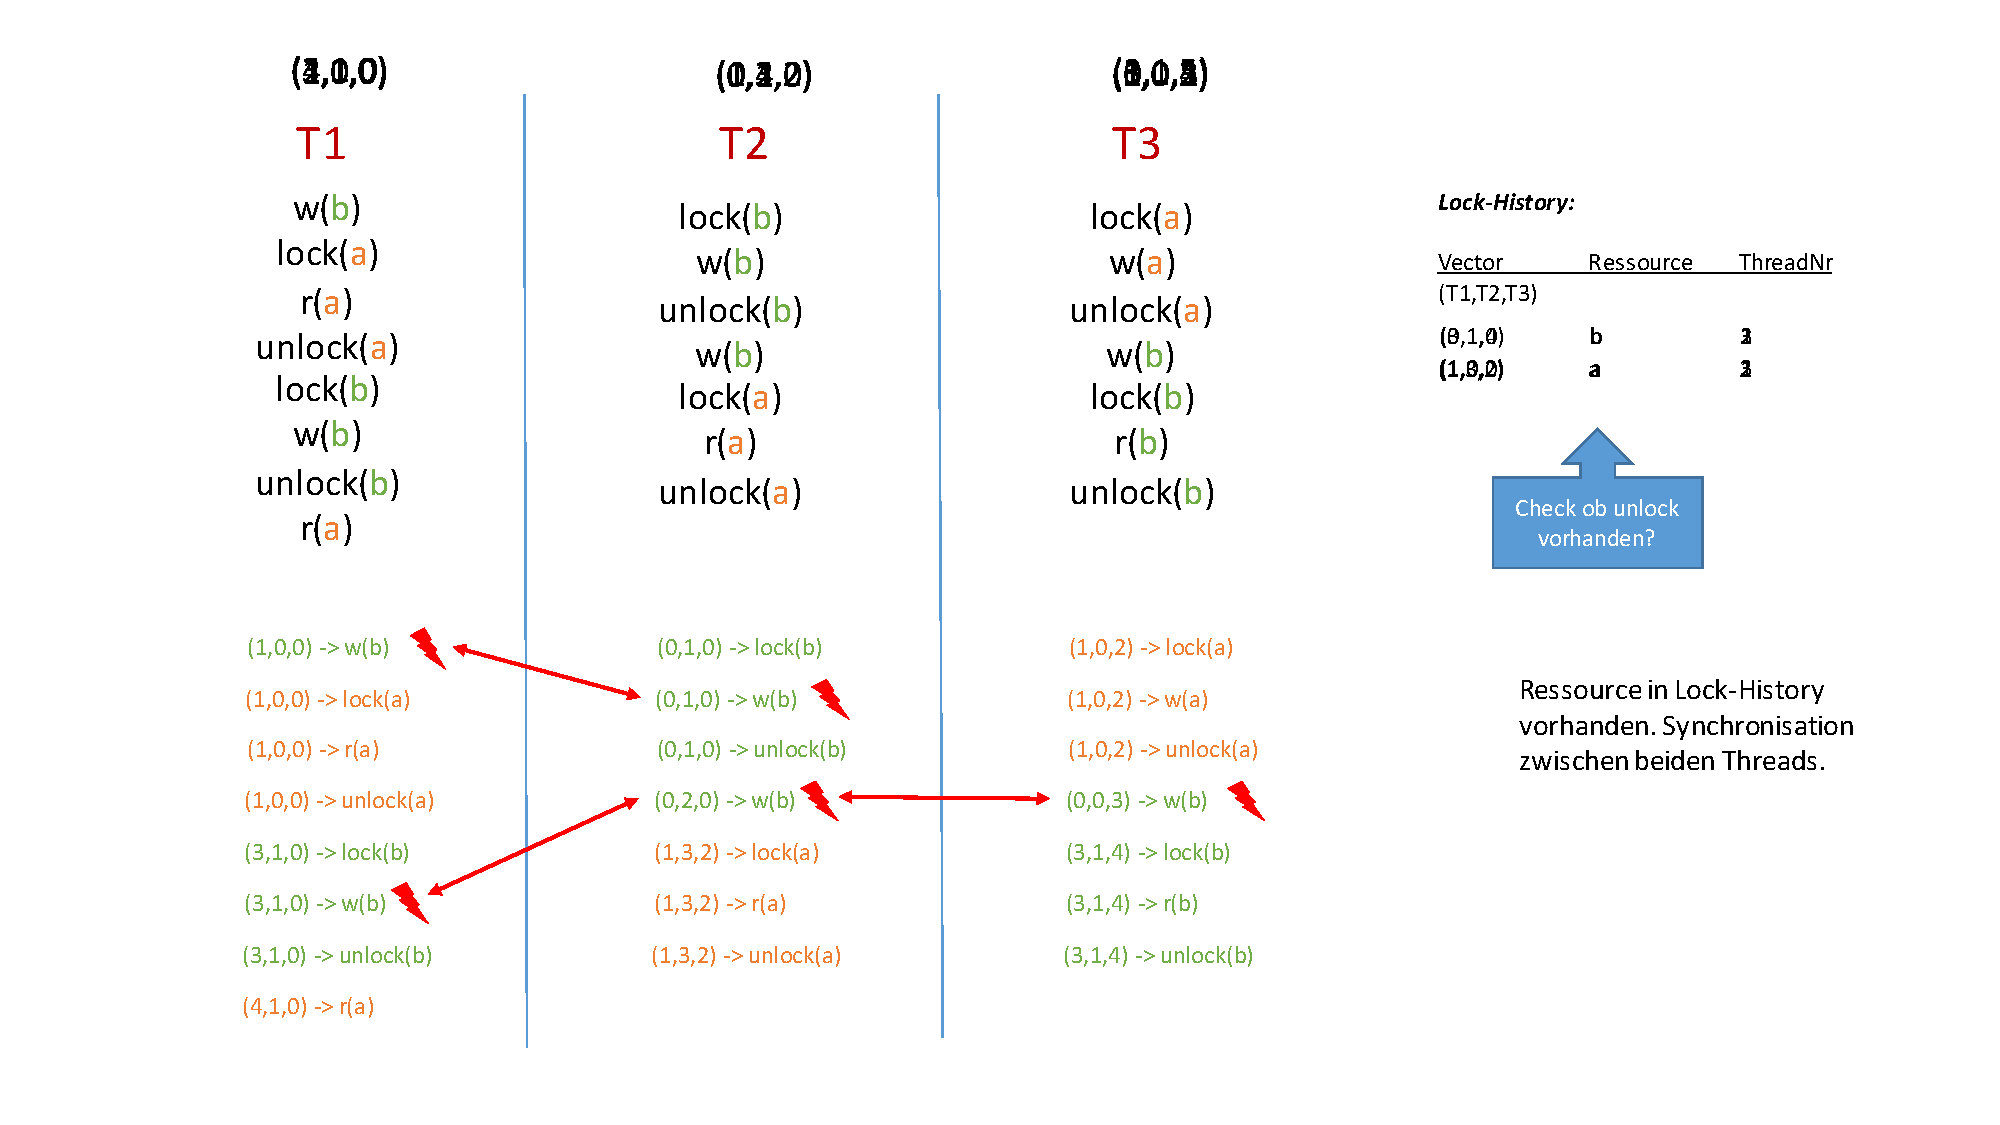
\includegraphics[width=14cm,height=5cm,trim=20mm 90mm 110mm 20mm, clip]{pictures/VectorCheckingAlgorithm.pdf}\\
\end{flushleft}
\subsection{Vektor Clock pro Thread}
\begin{flushleft}
Die Vektor Clock eignet sich optimal für den Dynamic Parallel Checker. Jeder Thread erhält seine eigene Vektor Clock um die Ereignisse in eine Kausalordnung zu bringen. Bei einem lock und anschliessendem unlock auf die gleiche Ressource wird die Vektor Clock der beiden Threads synchronisiert.\\
Die Vektor Clock wird vorallem dann benötigt, wenn alle Threads auf Race Conditions untersucht werden. Dabei kann mit Hilfe der Vektor Clock genau gesagt werden ob zwei Ereignisse (Read oder Write) in der Happened-Before Beziehung stehen oder ob sie Concurrent sind. Nur wenn sie Concurrent sind kann eine Race Condition aufgetreten sein.
\end{flushleft}
\subsection{Lock-History}
\begin{flushleft}
Während der kompletten Überprüfung wird eine Lock-History geführt, in der ersichtlich ist welcher Thread auf welche Ressource zu welcher Zeit (Vektor Clock) einen Lock durchgeführt hat. Diese History wird benötigt um eine Synchronisation zwischen zwei Threads vorzunehmen. Eine Lock-History könnte wie folgt aussehen:
\end{flushleft}
\begin{center}
\textbf{\textit{Lock-History:}}\\[0.5cm]
\begin{tabular}{ c c c }
  Vektor & Ressource & ThreadNr \\\hline
  (0,1,0) & b & 2 \\
  (1,0,0) & a & 1 \\\hline
\end{tabular}
\end{center}
\subsubsection{Synchronisation der Vektor Clock}
\begin{flushleft}
Wenn z.B. in unserem Beispielprogramm Thread1(T1) vor Thread3(T3) in den lock(a) Bereich kommt, schreibt er beim Verlassen des gesicherten Bereichs einen Eintrag in die Lock-History. Wenn nun T3 den lock von a beziehen möchte schaut er zuerst in die Lock-History und synchronisiert seine Vektor Clock (a1,a2,a3) mit der Vektor Clock des Eintrags in der Tabelle (b1,b2,b3).\\
Die neue Vektor Clock von T3 lässt sich nun wie folgt bilden: 
\begin{center}(b1, max(a2, b2), a3 + 1)\end{center}
\textit{Erklärung:}
\begin{itemize}
\item Von dem Thread, dessen Eintrag in der Lock-History zu einer Synchronisation führte, kann direkt der Wert übernommen werden.
\item Der synchronisierende Thread kann den eigenen Wert übernehmen und die Zahl 1 addieren.
\item Von jedem Thread der nicht in die Synchronisation involviert ist kann max(a, b) genommen werden.
\end{itemize}
Nach der Synchronisation ist eine Barriere aufgebaut. Kein Ereignis von T3 kann nach der Synchronisation mit einem Ereignis von T1 vor der Synchronisation in Konflikt stehen.
\end{flushleft}
\subsection{Funktion}
\begin{flushleft}

\end{flushleft}
\end{document}